\documentclass[border=3pt]{standalone}
% Preâmbulo compartilhado pelos diagramas TikZ da aula 5 de IHC (Processos de Design)
\usepackage[T1]{fontenc}
\usepackage[utf8]{inputenc}
\usepackage{lmodern}
\usepackage{amsmath}
\usepackage{xcolor}
\usepackage{tikz}
\usetikzlibrary{arrows.meta,angles,quotes,decorations.pathmorphing,calc,
                positioning,shapes.geometric,shapes.misc,backgrounds,fit,
                math}

% Paleta (mesma dos SVGs originais)
% Paleta da disciplina de IHC: acento roxo (#755099), da capa do livro.
% (o nome "dblue" é mantido para não alterar todos os diagramas)
\definecolor{dblue}{HTML}{755099}
\definecolor{dorange}{HTML}{B3541E}
\definecolor{dgreen}{HTML}{4A7C59}
\definecolor{dred}{HTML}{9C4B4B}
\definecolor{dcream}{HTML}{F4F1EA}
\definecolor{dshade}{HTML}{DDD7C9}

% Função gaussiana (não normalizada por padrão de escala visual)
\pgfmathdeclarefunction{gauss}{3}{%
  \pgfmathparse{1/(#3*sqrt(2*pi))*exp(-((#1-#2)^2)/(2*#3^2))}%
}

% Estilos comuns (prefixo d... para não colidir com chaves internas do pgf)
\tikzset{
  >={Stealth[length=2mm]},
  dguide/.style={gray!55, dashed, line width=0.4pt},
  daxis/.style={gray!60, line width=0.7pt, ->},
  dbody/.style={fill=black!3, draw=black!80, line width=1pt},
  dacc/.style={draw=dblue, line width=1pt},
  dlbl/.style={black!55, font=\small},
  dsub/.style={black!45, font=\footnotesize},
  dstate/.style={circle, draw=black!80, fill=dcream, line width=1pt,
                 minimum size=17mm, font=\large, inner sep=1pt},
  dobs/.style={circle, draw=black!80, fill=dshade, line width=1pt,
               minimum size=14mm, font=\large, inner sep=1pt},
  dbox/.style={rounded corners=2pt, draw=black!80, fill=dcream, line width=1pt,
               align=center, inner sep=6pt},
  dop/.style={circle, draw=black!80, fill=white, line width=1pt,
              minimum size=6mm, inner sep=0pt, font=\small},
  dtrans/.style={->, dblue, line width=1pt},
  dmeas/.style={->, dorange, line width=1pt},
  dcurve/.style={line width=1pt, dblue},
  dcurveb/.style={line width=1.4pt, dorange},
}

\begin{document}
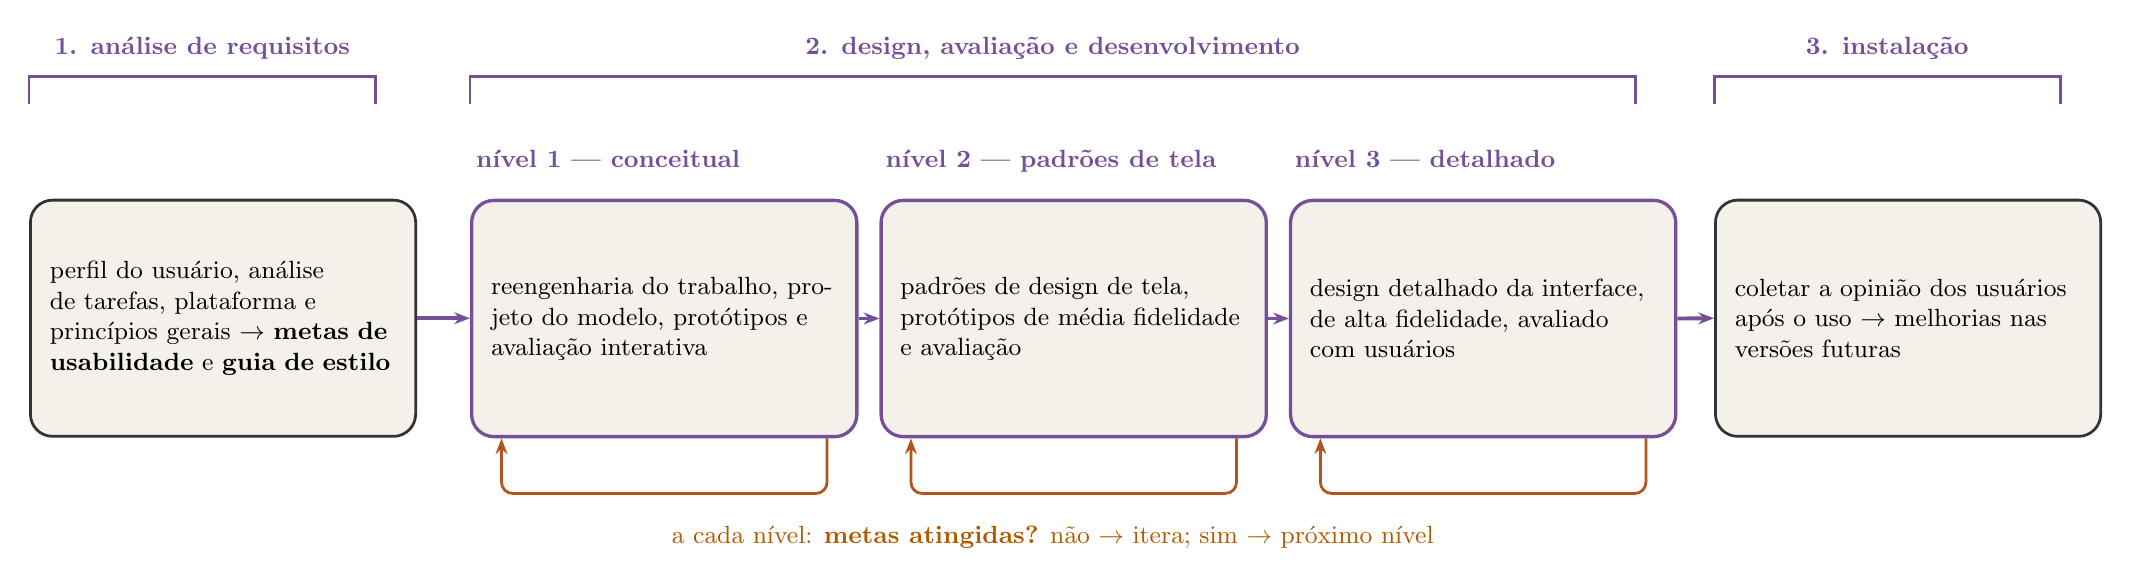
\begin{tikzpicture}[x=1cm,y=1cm,
   bx/.style={dbox, rounded corners=8pt, minimum height=3.0cm, text width=4.4cm, font=\small, align=left, inner sep=7pt, anchor=north west},
   tt/.style={font=\small\bfseries, text=dblue, text width=4.6cm, align=left, anchor=base west, inner sep=2pt}]

  % títulos (roxo), todos no mesmo nível, fora das caixas
  \node[tt] at (5.6,0.4) {nível 1 --- conceitual};
  \node[tt] at (10.8,0.4) {nível 2 --- padrões de tela};
  \node[tt] at (16.0,0.4) {nível 3 --- detalhado};

  % caixas, todas no mesmo nível
  \node[bx] (f1) at (0,0) {perfil do usuário, análise de tarefas, plataforma e princípios gerais $\to$ \textbf{metas de usabilidade} e \textbf{guia de estilo}};
  \node[bx, draw=dblue, line width=1.2pt] (n1) at (5.6,0) {reengenharia do trabalho, projeto do modelo, protótipos e avaliação interativa};
  \node[bx, draw=dblue, line width=1.2pt] (n2) at (10.8,0) {padrões de design de tela, protótipos de média fidelidade e avaliação};
  \node[bx, draw=dblue, line width=1.2pt] (n3) at (16.0,0) {design detalhado da interface, de alta fidelidade, avaliado com usuários};
  \node[bx] (f3) at (21.4,0) {coletar a opinião dos usuários após o uso $\to$ melhorias nas versões futuras};

  % as três fases, todas no mesmo nível (colchetes + títulos na mesma linha)
  \foreach \xa/\xb/\t in {0/4.4/{1. análise de requisitos}, 5.6/20.4/{2. design, avaliação e desenvolvimento}, 21.4/25.8/{3. instalação}} {
    \draw[dblue, line width=1pt] (\xa,1.2) -- (\xa,1.55) -- (\xb,1.55) -- (\xb,1.2);
    \node[font=\small\bfseries, text=dblue, anchor=south] at ({(\xa+\xb)/2},1.65) {\t};
  }

  \draw[dtrans, line width=1.4pt] (f1.east) -- (n1.west |- f1.east);
  \draw[dtrans, line width=1.4pt] (n1.east) -- (n2.west);
  \draw[dtrans, line width=1.4pt] (n2.east) -- (n3.west);
  \draw[dtrans, line width=1.4pt] (n3.east) -- (f3.west);

  % laços de iteração
  \foreach \n in {n1,n2,n3} {
    \draw[dmeas, rounded corners=4pt, line width=1pt] ([xshift=-0.4cm]\n.south east) -- ++(0,-0.7) -| ([xshift=0.4cm]\n.south west);
  }
  \node[dmeas, font=\small, orange!70!black] at (13.0,-4.3) {a cada nível: \textbf{metas atingidas?} não $\to$ itera; sim $\to$ próximo nível};

\end{tikzpicture}
\end{document}
